\chapter{Modelos de recuperación}\label{Chapter4} 
% chktex-file 8
% chktex-file 12
% chktex-file 13
% chktex-file 44

\section{Visión general}

Durante muchas décadas, los investigadores han diseñado varios tipos diferentes de modelos de recuperación que se dividen en diferentes categorías. Primero, una familia de los modelos se basa en la idea de similitud. Básicamente, se asume que si un documento es más similar a la consulta que otro documento, se diría que el primer documento es más relevante que el segundo. Entonces, en este caso, la función de clasificación se define como la similitud entre la consulta y el documento. Un ejemplo bien conocido de este caso es el modelo de espacio vectorial (Salton et al. 1975). \\

El segundo conjunto de modelos se llama modelos de recuperación probabilística. En esta familia de modelos, se sigue una estrategia muy diferente. Se asume que las consultas y los documentos son todas observaciones de variables aleatorias, y se asume que hay una variable aleatoria binaria llamada $R$ (con un valor de 1 o 0) para indicar si un documento es relevante para una consulta. Luego se define la puntuación de un documento con respecto a una consulta como la probabilidad de que esta variable aleatoria $R$ sea igual a 1 dado un documento y una consulta particulares. Hay diferentes casos de esta idea general. Uno es el modelo probabilístico clásico, que se remonta a trabajos realizados en las décadas de 1960 y 1970, otro es el enfoque de modelado de lenguaje, y otro más es el modelo de divergencia de la aleatoriedad. \\

Uno de los modelos de recuperación más efectivos derivados del marco de recuperación probabilística clásica es BM25 [Robertson y Zaragoza 2009], pero dado que la función de recuperación de BM25 es tan similar a un modelo de recuperación de espacio vectorial, se cubre como una variante del modelo de espacio vectorial. \\

El tercer tipo de modelo es la inferencia probabilística. Aquí la idea es asociar incertidumbre a las reglas de inferencia. Luego se puede cuantificar la probabilidad de poder demostrar que la consulta se deriva del documento. Esta familia de modelos es teóricamente atractiva, pero en la práctica, a menudo se reducen a modelos esencialmente similares al modelo de espacio vectorial o a un modelo de recuperación probabilística regular. \\

Finalmente, también hay una familia de modelos que utilizan el pensamiento axiomático. La idea es definir un conjunto de restricciones que se espera que satisfaga una buena función de recuperación. En este caso, el problema es encontrar una buena función de clasificación que pueda satisfacer todas las restricciones deseadas. \\

Aunque todos estos modelos se basan en diferentes pensamientos, al final las funciones de recuperación tienden a ser muy similares e involucran variables similares. El marco de recuperación axiomática ha demostrado ser efectivo para diagnosticar deficiencias de un modelo de recuperación y desarrollar modelos de recuperación mejorados en consecuencia (por ejemplo, BM25+ [Lv y Zhai 2011]).

\section{Forma general de la función de recuperación}

Antes de introducir modelos específicos, primero se verá la forma común de un modelo de recuperación de última generación y algunas de las ideas comunes utilizadas en todos estos modelos. Esto se ilustra en la figura \ref{fig:6.1}. Primero, estos modelos se basan en la suposición de usar una representación de bolsa de palabras (\textit{bag-of-words}) del texto. Una representación de bolsa de palabras sigue siendo la principal representación utilizada en todos los motores de búsqueda. Con esta suposición, la puntuación de una consulta como ``noticias de campaña presidencial'', con respecto a un documento $d$, se basaría en las puntuaciones calculadas en cada palabra individual de la consulta. Eso significa que la puntuación dependería de la puntuación de cada palabra, como ``presidencial'', ``campaña'' y ``noticias''. \\

\begin{figure}[h]
\centering
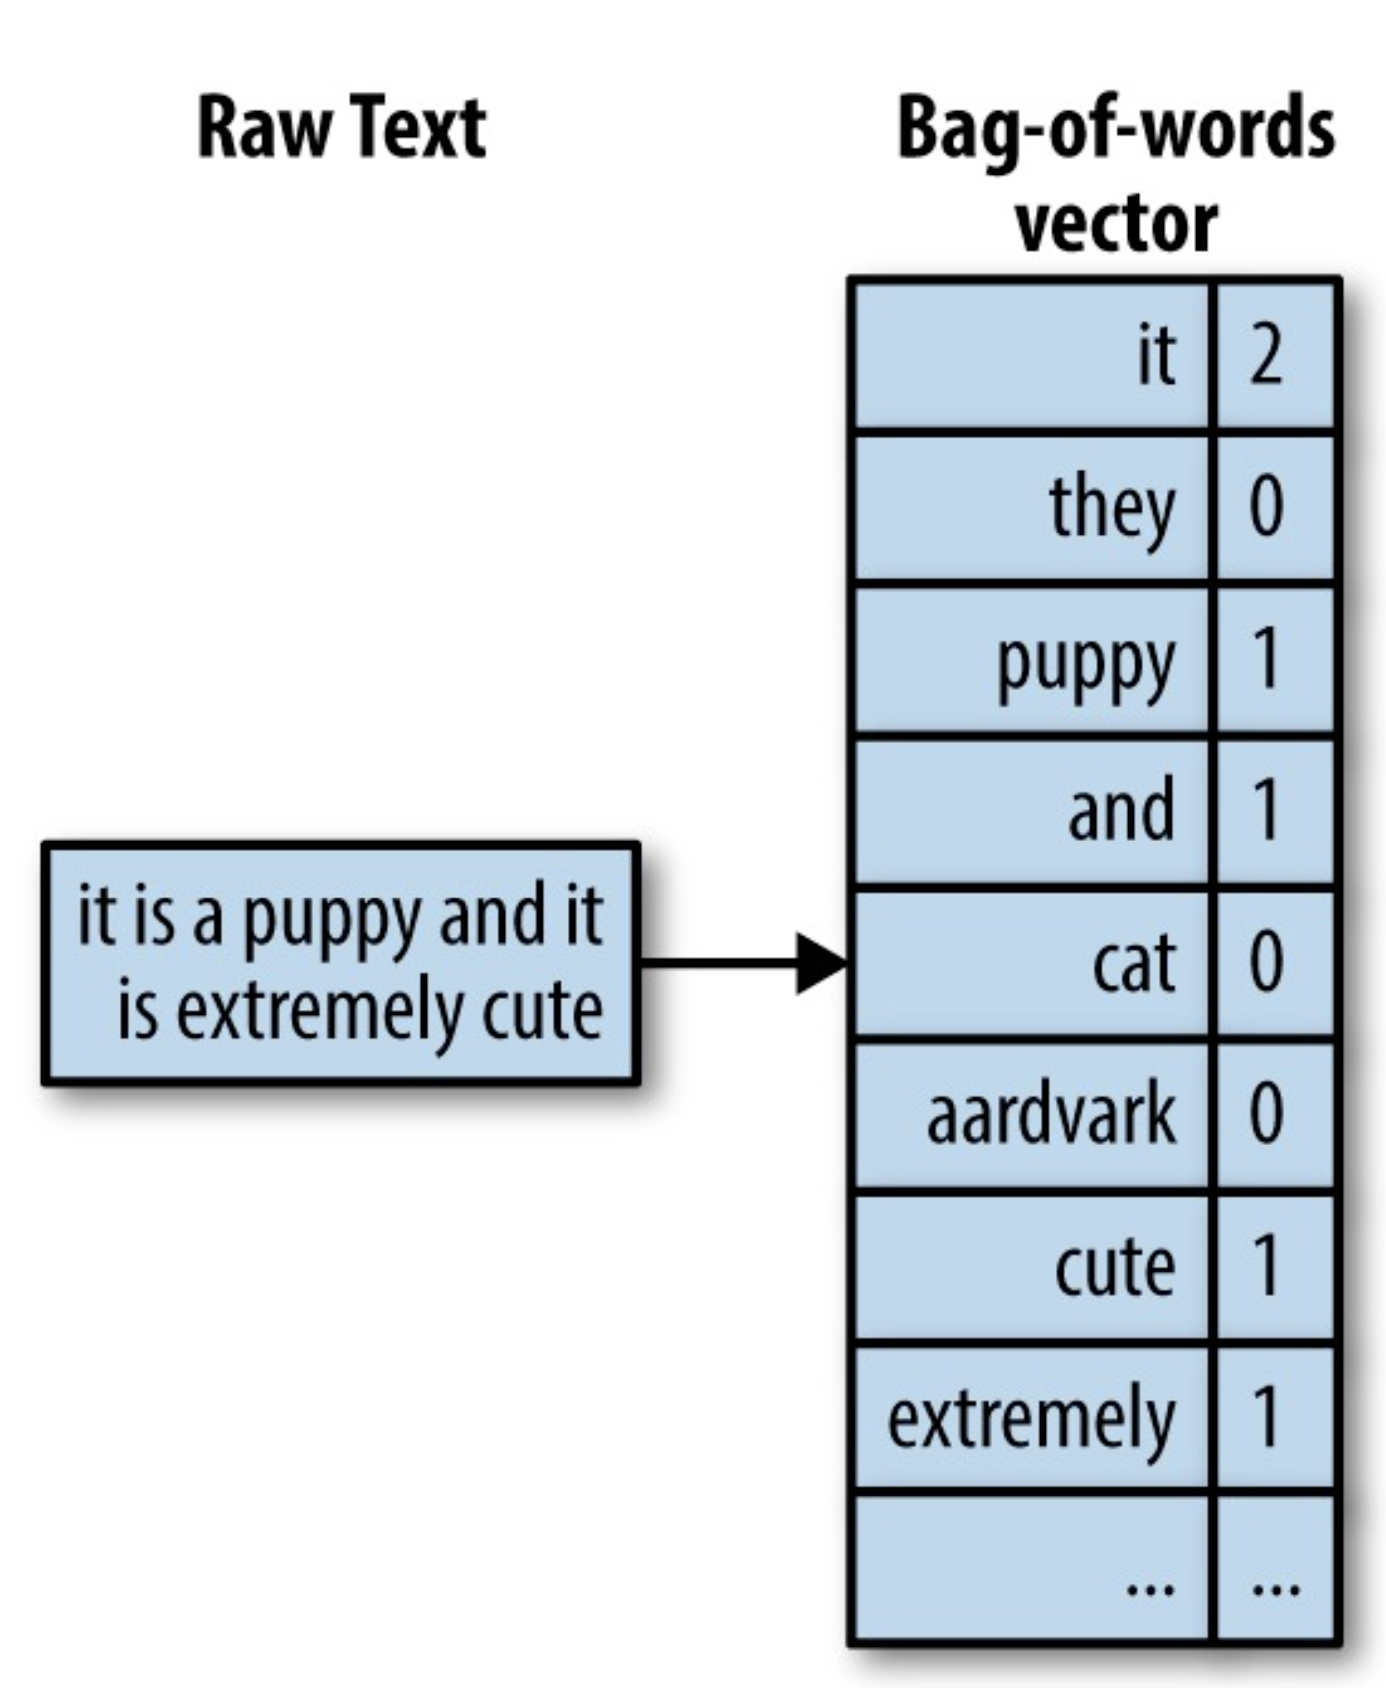
\includegraphics[width=0.3\textwidth]{fotos/15.png}
\caption{Bolsa de palabras}
\label{fig:6.0}
\end{figure}


Hay tres componentes diferentes, cada uno correspondiente a cómo de bien el documento coincide con cada una de las palabras de la consulta. Dentro de estas funciones, vemos una serie de heurísticas.
\begin{itemize}
\item  Un factor que afecta la función $g$ es cuántas veces ocurre la palabra ``presidencial'' en cada documento. Esto se llama frecuencia de término (TF). También podríamos denotar esto como $c(\text{presidencial}, d)$. En general, si la palabra ocurre con más frecuencia en el documento, el valor de esta función sería mayor. 
\item Otro factor es la longitud del documento (DL). En general, si un término ocurre muchas veces en un documento largo, no es tan significativo como si ocurriera el mismo número de veces en un documento corto (ya que se espera que cualquier término ocurra con más frecuencia en un documento largo). 
\item Finalmente, hay un factor llamado frecuencia de documento (DF). Esto observa con qué frecuencia ``presidencial'' ocurre al menos una vez en cualquier documento de toda la colección. Esto la frecuencia de documento, o DF, de ``presidencial''. DF intenta caracterizar la popularidad del término en la colección. En general, coincidir con un término raro en la colección contribuye más a la puntuación general que coincidir con un término común. 
\end{itemize}

TF, DF y DL capturan algunas de las ideas principales utilizadas en prácticamente todos los modelos de recuperación de última generación. En algunos otros modelos, también se usa una probabilidad para caracterizar esta información.

\begin{figure}[h]
\centering
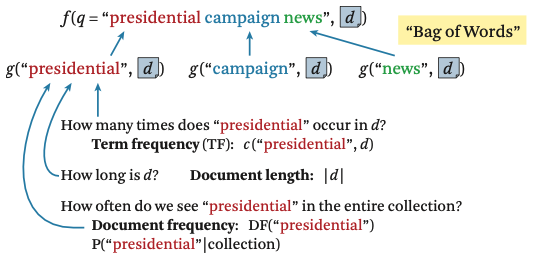
\includegraphics[width=0.6\textwidth]{fotos/16.png}
\caption{Ideas comunes para la puntuación con una representación de bolsa de palabras.}
\label{fig:6.1}
\end{figure}

Muchos modelos funcionan igual de bien, pero estos son los cuatro modelos principales que generalmente se consideran de última generación:
\begin{itemize}
\item Normalización de longitud pivotada (Singhal et al. 1996).
\item Okapi BM25 (Robertson y Zaragoza 2009).
\item Verosimilitud de consulta (\textit{query likelihood}) (Ponte y Croft 1998).
\item PL2 (Amati y Van Rijsbergen 2002).
\end{itemize}

En resumen, los puntos principales son los siguientes. Primero, el diseño de una buena función de clasificación requiere una definición computacional de relevancia, y se consigue este objetivo diseñando un modelo de recuperación adecuado. En segundo lugar, muchos modelos son igualmente efectivos, pero no existe un único ganador. Finalmente, las funciones de clasificación de última generación tienden a basarse en las siguientes ideas: 
\begin{itemize}
\item Representación de bolsa de palabras
\item TF y la frecuencia de documento de las palabras. 
\end{itemize}

Esta información es utilizada por una función de clasificación para determinar la contribución general de la coincidencia de una palabra, con un ajuste para la longitud del documento. Estas ideas a menudo se combinan.

\section{Modelos de recuperación de espacio vectorial}

\section{Modelos de recuperación de espacio vectorial}

El modelo de recuperación de espacio vectorial (VS) es un método simple pero efectivo para diseñar funciones de clasificación para la recuperación de información. Es un caso especial de los modelos basados en similitud, donde se asume que la relevancia está aproximadamente correlacionada con la similitud entre un documento y una consulta. En este proceso, inevitablemente hay que hacer una serie de suposiciones. Aquí se asume que si un documento es más similar a una consulta que otro documento, entonces se asumiría que el primer documento es más relevante que el segundo. Esta es la base para clasificar documentos en el modelo de espacio vectorial. Sin embargo, esta no es la única manera de formalizar la relevancia. \\

Sea un hiperespacio donde cada dimensión corresponde a un término; se pueden trazar los documentos en este espacio ya que están representados como vectores de magnitudes de términos. \\

\begin{figure}[h]
\centering
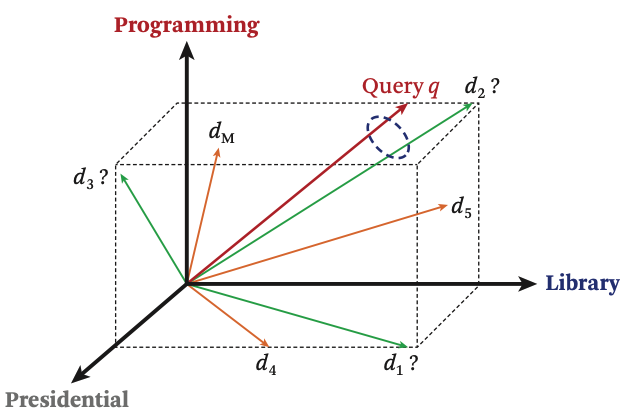
\includegraphics[width=0.7\textwidth]{fotos/17.png}
\caption{Espacio tridimensional con tres palabras: programación, biblioteca y presidencial.}
\label{fig:6.2}
\end{figure}

En la figura \ref{fig:6.2}, se tiene un espacio tridimensional con tres palabras: programación, biblioteca y presidencial; cada término define una dimensión. Se pueden considerar vectores en este espacio tridimensional, y se asume que todos los documentos y la consulta estarán ubicados en este espacio vectorial (es decir, es espacio es cerrado). Por ejemplo, el vector $d_1$ representa un documento que probablemente cubre los términos biblioteca y presidencial sin realmente hablar de programación. Para representar esl documento original se usa únicamente este vector, ignorando todo lo demás, incluyendo, por ejemplo, el orden de las palabras. No es una representación óptima, pero a menudo es suficiente para muchos problemas de recuperación. \\

Al usar esta representación de espacio vectorial, se pueden capturar intuitivamente las diferencias entre los temas de los documentos. De manera similar, se puede colocar la consulta en este espacio como otro vector y medir la similitud entre el vector de la consulta y cada vector de documento. En este caso, por ejemplo, podemos ver fácilmente que $d_2$ parece ser el más cercano al vector de la consulta y, por lo tanto, $d_2$ se clasificará por encima de los demás. Esta es la idea principal del modelo de espacio vectorial. \\

Para ser más precisos, el modelo VS es un marco. En este marco, se hacen algunas suposiciones. Una suposición es que se representará cada documento y consulta mediante un vector de términos. Aquí, un término puede ser cualquier concepto básico como una palabra o una frase, o incluso n-gramas de caracteres o cualquier otra representación de características. Se asume que cada término define una dimensión. Por lo tanto, dado que existen $|V|$ términos en el vocabulario, se define un espacio de $|V|$ dimensiones. Un vector de consulta consistiría en una serie de elementos correspondientes a los pesos de diferentes términos. Cada vector de documento es también similar; tiene una serie de elementos y cada valor de cada elemento indica el peso del término correspondiente. La relevancia en este caso se mide en función de la similitud entre los dos vectores. Por lo tanto, la función de recuperación también se define como la similitud entre el vector de la consulta y el vector del documento. \\

Para sugerir realmente una función particular que pueda implementarse, hay que refinar los conceptos anteriores. 
\begin{itemize}
\item Se asume que los conceptos son ortogonales, de lo contrario habrá redundancia (por ejemplo, si dos sinónimos se distinguen de alguna manera como dos conceptos diferentes, se definirían en dos dimensiones diferentes, causando una redundancia o sobreénfasis de la coincidencia de este concepto, ya que sería como si coincidieras con dos dimensiones cuando en realidad coincidiste con un solo concepto semántico). 
\item No se especifica cómo definir los pesos de los términos. El peso del término en el vector de la consulta indica la importancia de un término; dependiendo de cómo se asigne, se puede preferir que algunos términos coincidan sobre otros. De manera similar, el peso del término en el documento también es muy significativo: indica qué tan bien caracteriza el término al documento.
\item Finalmente, cómo definir la medida de similitud también es poco claro. 
\end{itemize}

\subsection{Modelo de espacio vectorial simple}

En la figura \ref{fig:6.3}, se ilustra la instanciación más simple del modelo de espacio vectorial. Aquí, se usa cada palabra del vocabulario para definir una dimensión, lo que da $|V|$ dimensiones: esta es la instanciación de bolsa de palabras. Para colocar los vectores en este espacio, la estrategia más simple es usar un vector de bits para representar tanto una consulta como un documento, y eso significa que cada elemento $x_i$ y $y_i$ tomaría un valor de cero o uno: cuando es uno, significa que la palabra correspondiente está presente en el documento o consulta; cuando es cero, está ausente. El vector de documento en general tendría más unos que el vector de consulta, pero aún habrá muchos ceros al ser el vocabulario muy extenso (de forma general). \\

\begin{figure}[h]
\centering
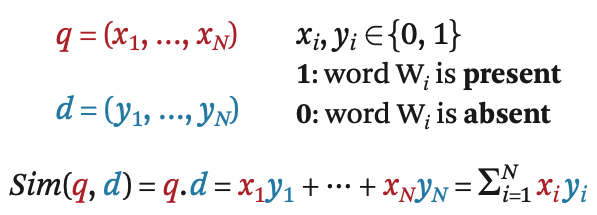
\includegraphics[width=0.5\textwidth]{fotos/18.png}
\caption{Cálculo de similitud entre una consulta y un vector de documento usando una representación de vector de \textit{bits} y el producto escalar como similitud.}
\label{fig:6.3}
\end{figure}

Una medida de similitud comúnmente utilizada es el producto escalar (cuenta el número de términos que coinciden, cuantos términos únicos de la consulta están presentes en el documento). Finalmente, se puede implementar una función de clasificación usando un lenguaje de programación y luego clasificar documentos en un corpus dada una consulta particular. \\

Para evaluar si este modelo de espacio vectorial más simple realmente funciona bien, se muestra un ejemplo en la figura \ref{fig:6.4}.

\begin{figure}[h]
\centering
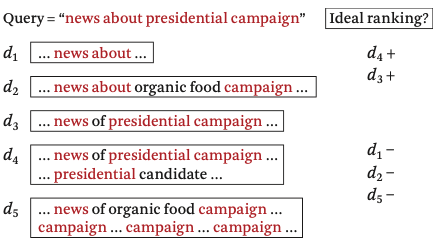
\includegraphics[width=0.5\textwidth]{fotos/19.png}
\caption{Aplicación de modelo VS de vector de bits e un ejemplo simple.}
\label{fig:6.4}
\end{figure}

Esta figura muestra algunos documentos de prueba y una consulta simple. La consulta es ``noticias sobre la campaña presidencial''. Para este ejemplo, se verán cinco documentos del corpus que cubren diferentes términos en la consulta. La clasificación ideal es la que haría el propio usuario, $R'(q)$. La mayoría de los usuarios estarían de acuerdo en que $d_4$ y $d_3$ probablemente son mejores que los otros, ya que estos dos realmente cubren bien la consulta. Coinciden con ``noticias'', ``presidencial'' y ``campaña'', por lo que deberían clasificarse en la parte superior. Los otros tres, $d_1$, $d_2$ y $d_5$, no son relevantes. \\

\begin{figure}[h]
\centering
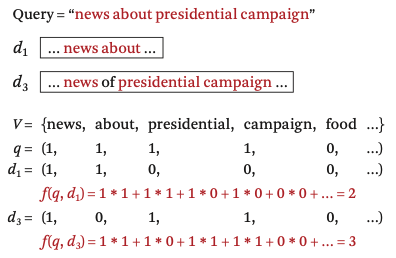
\includegraphics[width=0.5\textwidth]{fotos/20.png}
\caption{Cálculo del modelo de recuperación de vector de \textit{bits} en una consulta y el corpus.}
\label{fig:6.5}
\end{figure}

Ahora hay que ver si el modelo de espacio vectorial podría hacer lo mismo o algo cercano a la clasificación ideal. En la figura \ref{fig:6.5}, se muestran dos documentos, $d_1$ y $d_3$, junto con la consulta. En el modelo de espacio vectorial, primero se calculan los vectores para estos documentos y la consulta. La consulta tiene cuatro palabras, por lo que para estas cuatro palabras, habría un uno y para el resto habrá ceros. El documento $d_1$ tiene dos unos, ``noticias'' y ``sobre'', mientras que el resto de las dimensiones son ceros. Con los dos vectores, se puede calcular la similitud con el producto escalar, multiplicando los elementos correspondientes en cada vector. Cada par de vectores forma un producto, que representa la similitud entre los dos elementos. En este caso, el resultado será dos. Eso significa que este número es el valor de esta función de puntuación; es simplemente el recuento de cuántos términos únicos de la consulta coinciden en el documento. \\

Sin embargo, examinando este modelo en detalle, se encuentran algunos problemas. La función de puntuación cuenta el número de términos únicos de la consulta que coinciden en cada documento. Si un documento coincide con más términos únicos de la consulta, entonces se asumirá que el documento es más relevante; eso parece tener sentido. El único problema es que hay tres documentos, $d_2$, $d_3$ y $d_4$, que están empatados con una puntuación de tres. Al inspeccionar más de cerca, parece que $d_4$ debería estar justo por encima de $d_3$ ya que $d_3$ solo mencionó ``presidencial'' una vez mientras que $d_4$ lo mencionó muchas más veces. Otro problema es que $d_2$ y $d_3$ también tienen la misma puntuación, ya que para $d_2$, ``noticias'', ``sobre'' y ``campaña'' coincidieron. En $d_3$, coincidieron ``noticias'', ``presidencial'' y ``campaña''. Intuitivamente, $d_3$ es más relevante y debería tener una puntuación más alta que $d_2$. Coincidir con ``presidencial'' es más importante que coincidir con ``sobre'' aunque ``sobre'' y ``presidencial'' estén ambos en la consulta.

\subsubsection{Modelo VSP mejorado}

